\documentclass[11pt,a4paper]{article}

\usepackage[utf8]{inputenc}
\usepackage[T1]{fontenc}
\usepackage[brazil]{babel}
\usepackage{lmodern}
\usepackage[margin=2.5cm]{geometry}
\usepackage{graphicx}
\usepackage{booktabs}
\usepackage{amsmath,amssymb}
\usepackage{float}
\usepackage{caption}
\usepackage{subcaption}
\usepackage{listings}
\usepackage{xcolor}
\usepackage[hidelinks]{hyperref}

\captionsetup{font=small,labelfont=bf}
\graphicspath{{figuras/}}

\lstset{
  language=Java, basicstyle=\ttfamily\footnotesize, keywordstyle=\color{blue!60!black}\bfseries,
  commentstyle=\color{gray}\itshape, stringstyle=\color{orange!70!black}, frame=single,
  rulecolor=\color{gray!40}, numbers=left, numberstyle=\tiny\color{gray}, breaklines=true,
  showstringspaces=false, inputencoding=utf8, extendedchars=true,
  literate={á}{{\'a}}1 {ã}{{\~a}}1 {é}{{\'e}}1 {ê}{{\^e}}1 {í}{{\'i}}1 {ó}{{\'o}}1 {õ}{{\~o}}1 {ú}{{\'u}}1 {ç}{{\c{c}}}1
}

% ---------------------------------------------------------------
% Preencha com o(s) nome(s) completo(s) da dupla
\newcommand{\autores}{Saullo \\ \small Engenharia de Computação -- UNIPAMPA, campus Bagé}
% ---------------------------------------------------------------

\title{\textbf{Avaliação Experimental de Algoritmos de Ordenação em Java}\\[4pt]
\large Trabalho Prático 1 -- Algoritmos e Classificação de Dados}
\author{\autores}
\date{Outubro de 2026}

\begin{document}
\maketitle

\begin{abstract}
Este trabalho implementa em Java dez algoritmos de ordenação --- sete baseados em comparação
(Bubble, Insertion, Selection, Shell, Heap, Merge e Quick Sort) e três de tempo linear
(Counting, Radix e Bucket Sort) --- e avalia experimentalmente seu desempenho. Foram realizadas
3.850 medições de tempo, com vetores de $10^3$ a $10^7$ inteiros em ordem crescente, decrescente e
aleatória, com 10 a 30 repetições por configuração. Como extensão, cada algoritmo de comparação foi
implementado em duas versões: uma genérica, sobre \texttt{Comparable<T>}, e outra especializada para
o tipo primitivo \texttt{int}. Os resultados confirmam as ordens de crescimento previstas
(expoentes empíricos próximos de 2 para os quadráticos e de 1 para os demais) e o efeito do
melhor e do pior caso no Insertion e no Bubble Sort, mas mostram também que fatores ausentes da
análise assintótica --- hierarquia de memória, previsão de desvios e o custo da abstração genérica
(de $1{,}6\times$ a $24\times$) --- determinam boa parte dos tempos observados.
\end{abstract}

% ===============================================================
\section{Introdução}
% ===============================================================

Ordenar uma sequência de elementos é um dos problemas mais estudados da computação, tanto por sua
utilidade direta quanto por servir de etapa para outros algoritmos (busca binária, eliminação de
duplicatas, junções em bancos de dados etc.). A análise assintótica classifica os algoritmos de
ordenação em grandes famílias: os métodos elementares, com custo $\Theta(n^2)$; os métodos
eficientes por comparação, com custo $\Theta(n \log n)$, que é o limite inferior para qualquer
ordenação baseada em comparações; e os métodos que não comparam elementos, que atingem tempo linear
quando a entrada satisfaz certas condições.

A notação assintótica, porém, descarta constantes e termos de menor ordem, e não descreve o
comportamento da máquina real (memória cache, previsão de desvios, máquina virtual Java). O objetivo
deste trabalho é verificar experimentalmente até que ponto as previsões teóricas se confirmam
numa implementação concreta, e identificar quais características da implementação e da entrada
explicam as diferenças observadas. Especificamente, buscou-se:
\begin{itemize}
  \item implementar e verificar a corretude dos dez algoritmos;
  \item medir os tempos de execução para diferentes tamanhos e ordenações da entrada;
  \item comparar o crescimento observado com as complexidades teóricas;
  \item comparar algoritmos de mesma complexidade entre si;
  \item avaliar o custo da implementação genérica (\texttt{Comparable}) em relação ao tipo primitivo \texttt{int}.
\end{itemize}

% ===============================================================
\section{Algoritmos analisados}
% ===============================================================

A Tabela~\ref{tab:complexidades} resume as complexidades teóricas. Todos os algoritmos foram
implementados pelos autores; métodos prontos da API Java (\texttt{Arrays.sort}) foram usados apenas
para preparar entradas ordenadas e como oráculo nos testes, nunca no lugar das implementações.

\begin{table}[htbp]\centering\small
\caption{Complexidade de tempo e características dos algoritmos implementados}\label{tab:complexidades}
\setlength{\tabcolsep}{3.5pt}\footnotesize
\begin{tabular}{lllllcc}
\toprule
Algoritmo & Melhor caso & Caso médio & Pior caso & Memória extra & Estável & In-place \\
\midrule
Bubble    & $\Theta(n)$         & $\Theta(n^2)$       & $\Theta(n^2)$        & $O(1)$       & sim & sim \\
Insertion & $\Theta(n)$         & $\Theta(n^2)$       & $\Theta(n^2)$        & $O(1)$       & sim & sim \\
Selection & $\Theta(n^2)$       & $\Theta(n^2)$       & $\Theta(n^2)$        & $O(1)$       & não & sim \\
Shell     & $\Theta(n\log n)$   & $\approx n^{1{,}25}$ (emp.) & $O(n^{3/2})$ & $O(1)$       & não & sim \\
Heap      & $\Theta(n\log n)$   & $\Theta(n\log n)$   & $\Theta(n\log n)$    & $O(1)$       & não & sim \\
Merge     & $\Theta(n\log n)$   & $\Theta(n\log n)$   & $\Theta(n\log n)$    & $\Theta(n)$  & sim & não \\
Quick     & $\Theta(n\log n)$   & $\Theta(n\log n)$   & $\Theta(n^2)$        & $O(\log n)$ (pilha) & não & sim \\
\midrule
Counting  & \multicolumn{3}{c}{$\Theta(n+k)$}                               & $\Theta(n+k)$ & sim & não \\
Radix (LSD) & \multicolumn{3}{c}{$\Theta(d\,(n+b))$}                        & $\Theta(n+b)$ & sim & não \\
Bucket    & $\Theta(n)$         & $\Theta(n)$ (dist. uniforme) & $\Theta(n^2)$ & $\Theta(n)$  & sim & não \\
\bottomrule
\end{tabular}
\end{table}

\subsection{Algoritmos baseados em comparação}

\textbf{Bubble Sort} percorre o vetor trocando pares adjacentes fora de ordem; após a $i$-ésima
passada, os $i$ maiores elementos estão na posição final. A implementação usa um indicador de
troca: se uma passada não realiza trocas o vetor já está ordenado e o algoritmo termina, o que
dá melhor caso $\Theta(n)$.

\textbf{Insertion Sort} insere cada elemento $a[i]$ na posição correta do prefixo já ordenado
$a[0..i-1]$, deslocando os maiores uma posição à direita. O número de deslocamentos é igual ao
número de inversões do vetor: zero no vetor crescente, $n(n-1)/2$ no decrescente e cerca de
$n^2/4$ no aleatório.

\textbf{Selection Sort} seleciona o menor elemento de $a[i..n-1]$ e o troca com $a[i]$. Realiza
sempre $n(n-1)/2$ comparações, independentemente da entrada, e no máximo $n-1$ trocas.

\textbf{Shell Sort} aplica Insertion Sort a subsequências de elementos separados por um salto $h$
decrescente. Foi usada a sequência de Knuth ($h = 1, 4, 13, 40, \dots$, com $h_{k+1} = 3h_k+1$),
cujo pior caso é $O(n^{3/2})$; o desempenho médio não tem fórmula fechada conhecida e é
aproximadamente $n^{1{,}25}$ na prática.

\textbf{Heap Sort} constrói um heap de máximo em $O(n)$ (procedimento \emph{bottom-up}) e, em
seguida, troca repetidamente a raiz com o último elemento e restaura o heap, em $\Theta(n \log n)$
em todos os casos.

\textbf{Merge Sort} (top-down) divide o vetor ao meio, ordena recursivamente as metades e as
intercala. O vetor auxiliar de tamanho $n$ é alocado uma única vez e reutilizado em todas as
intercalações.

\textbf{Quick Sort} particiona o vetor em torno de um pivô e ordena recursivamente as partes. O pivô
é escolhido pela \emph{mediana de três} ($a[lo]$, $a[meio]$, $a[hi]$), e a partição usa o esquema
de dois índices que se cruzam (Sedgewick), que trata bem chaves repetidas. Com essa escolha de
pivô, vetores já ordenados (crescente ou decrescente) deixam de ser o pior caso e passam a produzir
partições equilibradas.

Os sete algoritmos têm assinatura genérica, conforme recomendado no enunciado, por exemplo:
\begin{lstlisting}
public static <T extends Comparable<T>> void heapsort(T[] a, int n)
public static <T extends Comparable<T>> void quicksort(T[] a, int lo, int hi)
\end{lstlisting}

\subsection{Algoritmos de tempo linear e condições adotadas}\label{sec:lineares}

Os três algoritmos lineares não comparam elementos entre si: eles usam o \emph{valor} da chave como
índice. Por isso trabalham sobre \texttt{int[]} e exigem hipóteses sobre os dados.

\textbf{Counting Sort} conta as ocorrências de cada valor em $[0,k]$, acumula as contagens para obter
as posições finais e distribui os elementos num vetor de saída percorrendo a entrada de trás para
frente (o que garante estabilidade). \emph{Condição}: chaves inteiras não negativas e $k$
pequeno em relação a $n$; o custo é $\Theta(n+k)$ em tempo e memória.

\textbf{Radix Sort} (LSD) aplica um Counting Sort estável a cada dígito, do menos para o mais
significativo. Foi usada a base $b=10$. \emph{Condição}: chaves inteiras não negativas; o custo é
$\Theta(d\,(n+b))$, onde $d$ é o número de dígitos do maior valor.

\textbf{Bucket Sort} distribui os elementos em $n$ baldes de acordo com o valor
($\text{balde} = \lfloor v \cdot n / (\max+1) \rfloor$, equivalente a normalizar $v$ para $[0,1)$),
ordena cada balde com Insertion Sort e concatena. Para evitar listas encadeadas, os baldes são
segmentos contíguos de um vetor auxiliar, com tamanhos obtidos por uma contagem prévia.
\emph{Condição}: distribuição aproximadamente uniforme; nesse caso cada balde tem $O(1)$ elementos
em média e o custo esperado é $\Theta(n)$.

\paragraph{Condições do experimento.} Em todos os experimentos os valores são inteiros
uniformemente distribuídos em $[0, n)$. Isso satisfaz as três condições acima: $k = n-1 = O(n)$
para o Counting Sort; distribuição uniforme para o Bucket Sort; e chaves não negativas para o
Radix Sort. Há duas consequências importantes:
\begin{enumerate}
  \item Como $k$ cresce junto com $n$, o vetor de contagem do Counting Sort tem o mesmo tamanho da
        entrada (40\,MB para $n=10^7$).
  \item Como o maior valor é $n-1$, o número de dígitos é $d = \lceil \log_{10} n \rceil$. Nessas
        condições o Radix Sort na base 10 custa $\Theta(n \log n)$, e não $\Theta(n)$.
\end{enumerate}
A comparação com os algoritmos baseados em comparação é válida porque todos recebem exatamente os
mesmos vetores e porque as hipóteses dos lineares são satisfeitas. A comparação \emph{não} se
generaliza para chaves arbitrárias: com valores de 32 bits quaisquer, por exemplo, o Counting Sort
precisaria de um vetor de contagem de 16\,GB e seria inviável.

% ===============================================================
\section{Metodologia}
% ===============================================================

\subsection{Hardware e software}

\begin{table}[htbp]\centering\small
\caption{Ambiente de execução}\label{tab:ambiente}
\begin{tabular}{lp{11.2cm}}
\toprule
Processador & AMD Ryzen 7 5825U (Zen 3, 8 núcleos / 16 threads, até 4,5\,GHz; L2 512\,KB/núcleo, L3 16\,MB) \\
Computador hospedeiro & Notebook com Windows (x64) \\
Ambiente de execução & Máquina virtual Linux Ubuntu 22.04.5 LTS (kernel 6.8), 2 vCPUs, 2,8\,GB de RAM \\
Java & OpenJDK 11.0.32, HotSpot 64-Bit Server VM (compilador JIT C2) \\
Opções da JVM & \texttt{-Xmx2g -Xss512m} (heap de 2\,GB; pilha ampliada por segurança na recursão) \\
Compilação & \texttt{javac --release 11} \\
Análise & Python 3 (pandas, NumPy, Matplotlib) \\
\bottomrule
\end{tabular}
\end{table}

Os experimentos foram executados numa máquina virtual Linux sobre o notebook com Windows
(Tabela~\ref{tab:ambiente}). A virtualização e o gerenciamento de energia do notebook (variação de
frequência) são fontes de ruído que não puderam ser eliminadas; procurou-se reduzi-las mantendo
o computador sem outras tarefas pesadas durante as medições.

\subsection{Organização do código}

\begin{itemize}
  \item \texttt{Ordenadores.java}: os sete algoritmos de comparação, genéricos (\texttt{Comparable<T>});
  \item \texttt{OrdenadoresInt.java}: os mesmos sete, especializados para \texttt{int[]} (extensão);
  \item \texttt{OrdenadoresLineares.java}: Counting, Radix e Bucket Sort;
  \item \texttt{Algoritmo.java}: catálogo que permite chamar todos os algoritmos da mesma forma;
  \item \texttt{TesteCorretude.java}: testes da Etapa 1;
  \item \texttt{Experimento.java}: geração das entradas, medição e gravação dos tempos;
  \item \texttt{analise/analise.py}: estatísticas, gráficos e tabelas.
\end{itemize}

As versões genérica e \texttt{int} têm exatamente a mesma lógica (mesmas comparações, trocas e
escolha de pivô); muda apenas o tipo dos elementos. Isso permite isolar o custo da abstração.

\subsection{Verificação da corretude}

Os testes foram feitos em duas partes. Na \emph{parte A}, seis vetores pequenos com 10 a 15
elementos (tamanhos pares e ímpares) nos casos crescente, decrescente, aleatório e com muitas
repetições (incluindo um vetor com todos os elementos iguais) foram ordenados pelas 17
implementações (7 genéricas, 7 \texttt{int} e 3 lineares); os vetores antes e depois foram
registrados em \texttt{resultados/testes\_corretude.txt}. Na \emph{parte B}, complementar, 2.000
vetores aleatórios com tamanhos de 0 a 300 (um terço deles com valores em $[0,5)$, para forçar
repetições) foram ordenados por todas as implementações e comparados a um oráculo, totalizando
34.000 verificações. Todas passaram. Além disso, durante os experimentos, cada vetor ordenado foi
verificado (fora do trecho medido); nenhuma execução falhou.

\subsection{Dados de entrada}

Para cada tamanho $n$ foi gerado \emph{um} vetor de inteiros uniformes em $[0,n)$ com semente fixa
($20261018 + n$), o que torna o experimento reprodutível. A configuração crescente é esse mesmo
vetor ordenado, e a decrescente é ele invertido; assim, as três configurações têm exatamente os
mesmos valores, diferindo só na ordem --- detalhe relevante para os algoritmos lineares, cujo
custo depende dos valores. Para a versão genérica, o vetor é convertido para \texttt{Integer[]}.

Cada algoritmo recebe uma \emph{cópia} do vetor original a cada execução
(\texttt{original.clone()}), de modo que todos os algoritmos de uma configuração ordenam
exatamente a mesma entrada.

\subsection{Tamanhos e repetições}

O plano experimental (Tabela~\ref{tab:plano}) foi definido de modo a caber no tempo disponível:
os algoritmos quadráticos chegam a 40\,s por execução em $n=10^5$, o que torna $n=10^6$ inviável
(estimativa de mais de uma hora por execução).

\begin{table}[htbp]\centering\small
\caption{Plano experimental executado (3.850 medições no total)}\label{tab:plano}
\begin{tabular}{llll}
\toprule
Configuração & Algoritmos & Tamanhos $n$ & Repetições \\
\midrule
Aleatória & $n\log n$ (genérico e \texttt{int}) e lineares & $10^3, 10^4, 10^5, 10^6$ & 30 \\
Aleatória & $n\log n$ e lineares (só \texttt{int}) & $10^7$ & 10 \\
Aleatória & quadráticos (genérico e \texttt{int}) & $10^3,\ 5\cdot10^3,\ 10^4$ & 30 \\
Aleatória & quadráticos (genérico e \texttt{int}) & $5\cdot10^4,\ 10^5$ & 10 \\
Crescente / decrescente & todos & $10^4$ & 30 \\
Crescente / decrescente & quadráticos & $5\cdot10^4$ & 10 \\
Crescente / decrescente & $n\log n$ e lineares & $10^6$ & 30 \\
\bottomrule
\end{tabular}
\end{table}

\subsection{Procedimento de medição}

O código de medição (\texttt{Experimento.java}) segue, para cada combinação de implementação,
configuração e tamanho, os passos abaixo:
\begin{enumerate}
  \item \textbf{Aquecimento global da JVM}: no início de cada execução do programa, todos os
        algoritmos ordenam 15 vezes um vetor de 5.000 elementos, para que o compilador JIT
        otimize o código antes das medições. Esses tempos são descartados.
  \item \textbf{Aquecimento local}: antes das repetições medidas, cada algoritmo é executado de 1
        a 3 vezes sobre o vetor da configuração, também descartadas (exceto nos quadráticos com
        $n \ge 5\cdot10^4$, em que cada execução leva segundos e o aquecimento global basta).
  \item \textbf{Medição}: a cópia do vetor é criada e \texttt{System.gc()} é chamado
        \emph{antes} de iniciar o cronômetro, reduzindo a chance de uma coleta de lixo cair dentro
        da medição. Apenas a chamada de ordenação é medida:
\begin{lstlisting}
int[] v = original.clone();     // fora da medição
System.gc();                    // fora da medição
long inicio = System.nanoTime();
e.alg().ordena(v);
long fim = System.nanoTime();
// verificação e gravação também fora da medição
\end{lstlisting}
  \item \textbf{Registro}: cada tempo individual é gravado numa linha de
        \texttt{resultados/tempos.csv} com as colunas \texttt{impl, algoritmo, config, n, rep, tempo\_ns}.
\end{enumerate}

Para o Counting e o Bucket Sort, a busca do maior valor (necessária para dimensionar as estruturas)
é feita dentro da chamada medida, por fazer parte do algoritmo.

\subsection{Tratamento dos dados}

Para cada configuração foram calculados média, mediana, mínimo, máximo, desvio-padrão e
coeficiente de variação (CV = desvio/média), gravados em \texttt{resultados/estatisticas.csv}.
Nos gráficos de crescimento foi usada a \textbf{mediana}, por ser menos sensível a medições
isoladas muito altas (coletas de lixo, interferência do sistema). Nenhuma medição foi descartada.
Para comparar com a teoria, estimou-se o expoente empírico $b$ ajustando por mínimos quadrados a
reta $\log t = \log c + b \log n$ aos tamanhos $n \ge 10^4$. Para referência: se $t \propto n^2$,
$b = 2$; se $t \propto n \log n$, a inclinação local é $1 + 1/\ln n$, que vai de 1,11 ($n=10^4$) a 1,06 ($n=10^7$).

% ===============================================================
\section{Resultados}
% ===============================================================

As Tabelas~\ref{tab:int-aleat} e~\ref{tab:gen-aleat} apresentam os tempos médios em ordem
aleatória, e as Figuras~\ref{fig:quad} e~\ref{fig:nlogn} mostram o crescimento em escala log-log.
Nessa escala, uma função $c\,n^b$ aparece como uma reta de inclinação $b$.

\begin{table}[htbp]\centering\small
\caption{Tempo médio (ms) — implementação \texttt{int[]}, ordem aleatória}\label{tab:int-aleat}
\setlength{\tabcolsep}{4pt}
\begin{tabular}{lrrrrrrr}
\toprule
Algoritmo & 1.000 & 5.000 & 10.000 & 50.000 & 100.000 & 1.000.000 & 10.000.000 \\
\midrule
Bubble & 0,562 & 9,04 & 35,4 & 2.158 & 9.845 & -- & -- \\
Insertion & 0,091 & 1,60 & 5,81 & 144 & 596 & -- & -- \\
Selection & 0,253 & 4,44 & 16,5 & 423 & 1.780 & -- & -- \\
Shell & 0,051 & -- & 0,691 & -- & 8,48 & 121 & 1.756 \\
Heap & 0,046 & -- & 0,553 & -- & 7,30 & 106 & 3.026 \\
Merge & 0,076 & -- & 0,683 & -- & 7,39 & 90,6 & 1.103 \\
Quick & 0,063 & -- & 0,642 & -- & 6,92 & 80,6 & 906 \\
Counting & 0,014 & -- & 0,046 & -- & 0,523 & 21,7 & 920 \\
Radix & 0,039 & -- & 0,331 & -- & 3,50 & 47,7 & 593 \\
Bucket & 0,024 & -- & 0,117 & -- & 1,18 & 34,2 & 942 \\
\bottomrule
\end{tabular}
\end{table}
\begin{table}[htbp]\centering\small
\caption{Tempo médio (ms) — implementação genérica (\texttt{Comparable}), ordem aleatória}\label{tab:gen-aleat}
\setlength{\tabcolsep}{4pt}
\begin{tabular}{lrrrrrr}
\toprule
Algoritmo & 1.000 & 5.000 & 10.000 & 50.000 & 100.000 & 1.000.000 \\
\midrule
Bubble & 1,40 & 45,1 & 239 & 7.837 & 37.726 & -- \\
Insertion & 0,456 & 20,8 & 70,4 & 2.866 & 14.612 & -- \\
Selection & 0,510 & 10,1 & 39,6 & 1.423 & 6.678 & -- \\
Shell & 0,099 & -- & 1,90 & -- & 30,5 & 712 \\
Heap & 0,095 & -- & 1,53 & -- & 19,3 & 604 \\
Merge & 0,123 & -- & 1,32 & -- & 19,5 & 350 \\
Quick & 0,071 & -- & 1,01 & -- & 11,5 & 208 \\
\bottomrule
\end{tabular}
\end{table}

\begin{figure}[htbp]\centering
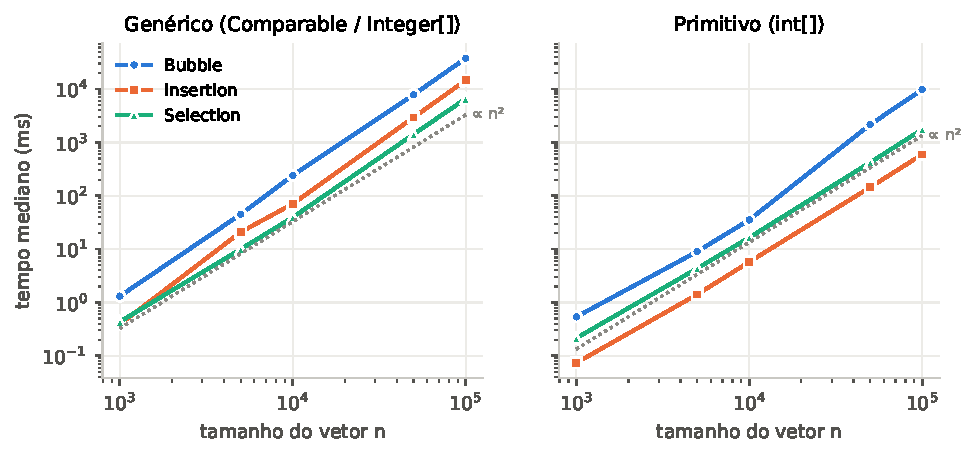
\includegraphics[width=\linewidth]{fig_quadraticos.pdf}
\caption{Algoritmos quadráticos, ordem aleatória (mediana, escala log-log). A reta pontilhada tem
inclinação 2.}\label{fig:quad}
\end{figure}

\begin{figure}[htbp]\centering
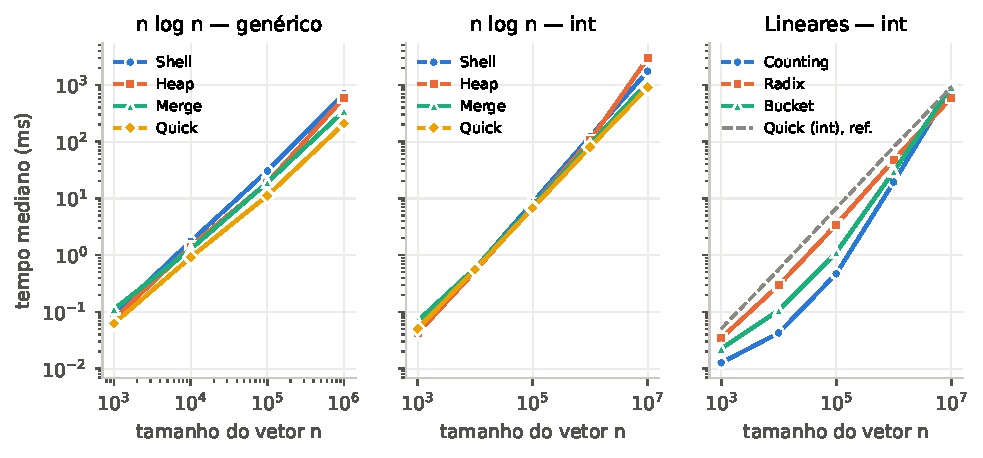
\includegraphics[width=\linewidth]{fig_nlogn_lineares.pdf}
\caption{Algoritmos $O(n\log n)$ e lineares, ordem aleatória (mediana, escala log-log). No painel
dos lineares, a linha tracejada é o Quick Sort \texttt{int} como referência.}\label{fig:nlogn}
\end{figure}

A Tabela~\ref{tab:expoentes} traz os expoentes empíricos, e a Figura~\ref{fig:norm} mostra o tempo
dividido pela função de complexidade teórica: se a previsão for exata, a curva é horizontal.

\begin{table}[htbp]\centering\small
\caption{Expoente empírico $b$ do ajuste $t \approx c\,n^b$ (ordem aleatória, $n \ge 10^4$)}\label{tab:expoentes}
\begin{tabular}{llrrr}
\toprule
Algoritmo & Complexidade (médio) & $b$ genérico & $b$ \texttt{int} & Faixa de $n$ (\texttt{int}) \\
\midrule
Bubble & $\Theta(n^2)$ & 2,19 & 2,46 & $10^{4}$--$10^{5}$ \\
Insertion & $\Theta(n^2)$ & 2,32 & 2,01 & $10^{4}$--$10^{5}$ \\
Selection & $\Theta(n^2)$ & 2,22 & 2,02 & $10^{4}$--$10^{5}$ \\
Shell & $\approx O(n^{3/2})$ & 1,30 & 1,16 & $10^{4}$--$10^{7}$ \\
Heap & $\Theta(n\log n)$ & 1,31 & 1,24 & $10^{4}$--$10^{7}$ \\
Merge & $\Theta(n\log n)$ & 1,22 & 1,09 & $10^{4}$--$10^{7}$ \\
Quick & $\Theta(n\log n)$ & 1,18 & 1,07 & $10^{4}$--$10^{7}$ \\
Counting & $\Theta(n+k)$ & -- & 1,46 & $10^{4}$--$10^{7}$ \\
Radix & $\Theta(d(n+b))$ & -- & 1,11 & $10^{4}$--$10^{7}$ \\
Bucket & $\Theta(n)$ & -- & 1,32 & $10^{4}$--$10^{7}$ \\
\bottomrule
\end{tabular}
\end{table}

\begin{figure}[htbp]\centering
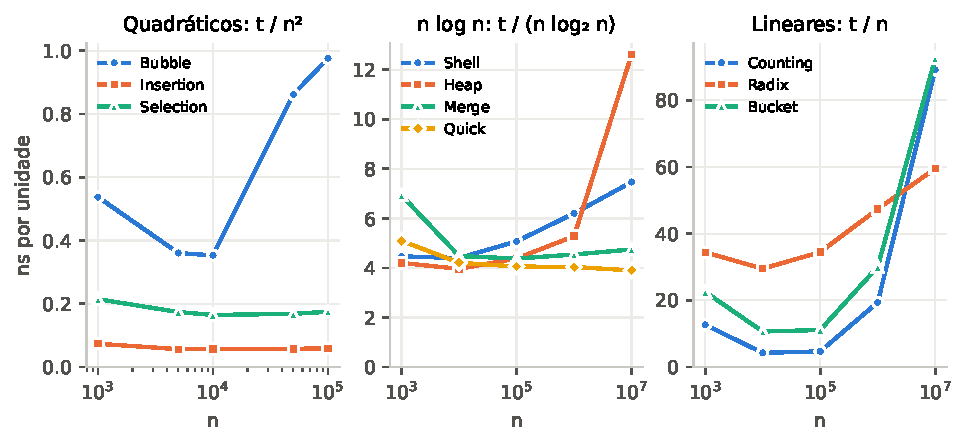
\includegraphics[width=\linewidth]{fig_normalizado.pdf}
\caption{Tempo normalizado pela complexidade teórica (\texttt{int[]}, ordem aleatória). Curvas
horizontais indicam concordância com a teoria.}\label{fig:norm}
\end{figure}

\subsection{Influência da ordem da entrada}

As Tabelas~\ref{tab:cfg-int-10k}--\ref{tab:cfg-gen-50k} e as Figuras~\ref{fig:cfg10k}
e~\ref{fig:cfg1M} comparam as três configurações. A última coluna das tabelas é a razão entre o
tempo no vetor decrescente e no aleatório.

\begin{table}[htbp]\centering\small
\caption{Tempo médio (ms) por configuração — \texttt{int[]}, $n = 10^4$}\label{tab:cfg-int-10k}
\begin{tabular}{lrrrr}
\toprule
Algoritmo & Crescente & Aleatória & Decrescente & Decresc./Aleat. \\
\midrule
Bubble & 0,012 & 35,4 & 22,0 & 0,62 \\
Insertion & 0,012 & 5,81 & 11,4 & 1,96 \\
Selection & 16,0 & 16,5 & 29,0 & 1,75 \\
Shell & 0,069 & 0,691 & 0,146 & 0,21 \\
Heap & 0,409 & 0,553 & 0,405 & 0,73 \\
Merge & 0,239 & 0,683 & 0,278 & 0,41 \\
Quick & 0,193 & 0,642 & 0,187 & 0,29 \\
Counting & 0,077 & 0,046 & 0,048 & 1,04 \\
Radix & 0,349 & 0,331 & 0,316 & 0,95 \\
Bucket & 0,134 & 0,117 & 0,105 & 0,90 \\
\bottomrule
\end{tabular}
\end{table}
\begin{table}[htbp]\centering\small
\caption{Tempo médio (ms) por configuração — genérico, $n = 10^4$}\label{tab:cfg-gen-10k}
\begin{tabular}{lrrrr}
\toprule
Algoritmo & Crescente & Aleatória & Decrescente & Decresc./Aleat. \\
\midrule
Bubble & 0,026 & 239 & 273 & 1,14 \\
Insertion & 0,051 & 70,4 & 131 & 1,86 \\
Selection & 41,9 & 39,6 & 46,1 & 1,16 \\
Shell & 0,309 & 1,90 & 0,470 & 0,25 \\
Heap & 0,856 & 1,53 & 0,815 & 0,53 \\
Merge & 0,742 & 1,32 & 0,808 & 0,61 \\
Quick & 0,293 & 1,01 & 0,313 & 0,31 \\
\bottomrule
\end{tabular}
\end{table}
\begin{table}[htbp]\centering\small
\caption{Tempo médio (ms) por configuração — quadráticos \texttt{int[]}, $n = 5\cdot10^4$}\label{tab:cfg-int-50k}
\begin{tabular}{lrrrr}
\toprule
Algoritmo & Crescente & Aleatória & Decrescente & Decresc./Aleat. \\
\midrule
Bubble & 0,211 & 2.158 & 1.143 & 0,53 \\
Insertion & 0,227 & 144 & 313 & 2,17 \\
Selection & 550 & 423 & 2.130 & 5,04 \\
\bottomrule
\end{tabular}
\end{table}
\begin{table}[htbp]\centering\small
\caption{Tempo médio (ms) por configuração — quadráticos genérico, $n = 5\cdot10^4$}\label{tab:cfg-gen-50k}
\begin{tabular}{lrrrr}
\toprule
Algoritmo & Crescente & Aleatória & Decrescente & Decresc./Aleat. \\
\midrule
Bubble & 0,361 & 7.837 & 7.854 & 1,00 \\
Insertion & 0,331 & 2.866 & 4.596 & 1,60 \\
Selection & 1.256 & 1.423 & 2.644 & 1,86 \\
\bottomrule
\end{tabular}
\end{table}

\begin{figure}[htbp]\centering
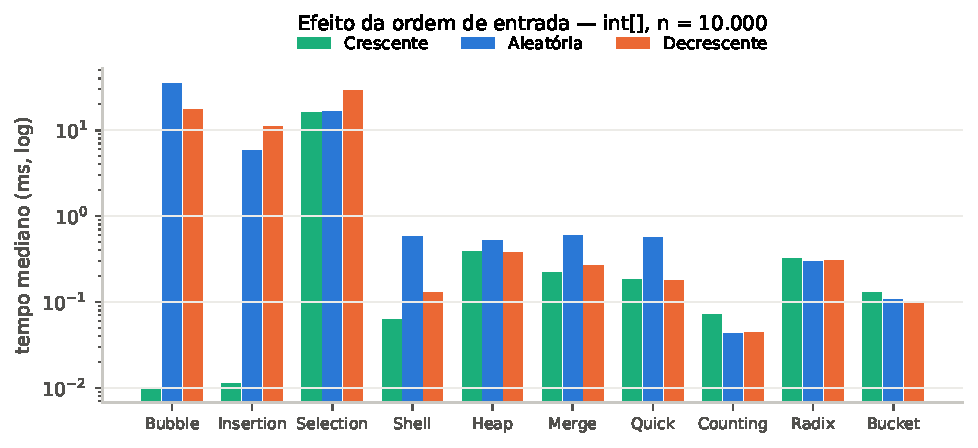
\includegraphics[width=\linewidth]{fig_config_int_10k.pdf}
\caption{Efeito da ordem da entrada, \texttt{int[]}, $n=10^4$ (escala logarítmica).}\label{fig:cfg10k}
\end{figure}

\begin{figure}[htbp]\centering
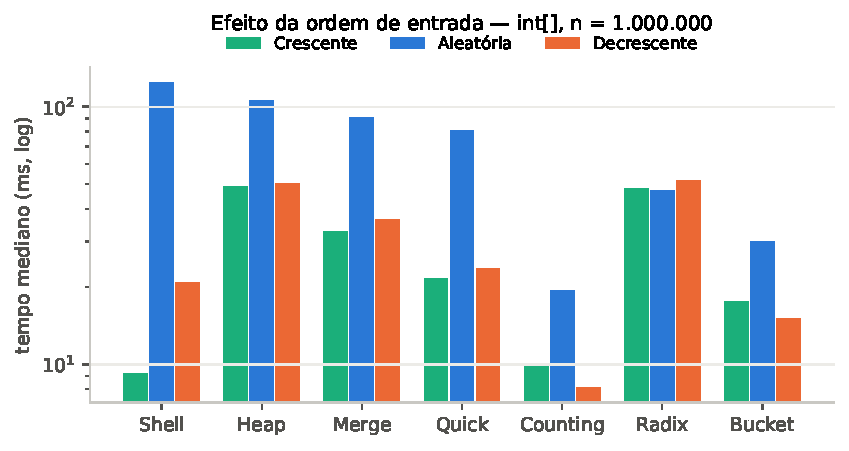
\includegraphics[width=0.88\linewidth]{fig_config_int_1M.pdf}
\caption{Efeito da ordem da entrada, \texttt{int[]}, $n=10^6$ (escala logarítmica).}\label{fig:cfg1M}
\end{figure}

\subsection{Variabilidade entre execuções}

As Tabelas~\ref{tab:det-int-1M} e~\ref{tab:det-gen-100k} trazem todas as estatísticas de duas
configurações representativas, e a Figura~\ref{fig:box} mostra a distribuição das repetições em
boxplots.

\begin{table}[htbp]\centering\small
\caption{Estatísticas completas (ms) — \texttt{int[]}, ordem aleatória, $n = 10^6$}\label{tab:det-int-1M}
\begin{tabular}{lrrrrrrr}
\toprule
Algoritmo & Rep. & Média & Mediana & Mín. & Máx. & Desvio & CV (\%) \\
\midrule
Shell & 30 & 121 & 124 & 114 & 126 & 3,85 & 3,2 \\
Heap & 30 & 106 & 105 & 99,9 & 118 & 4,04 & 3,8 \\
Merge & 30 & 90,6 & 90,5 & 88,9 & 92,8 & 1,03 & 1,1 \\
Quick & 30 & 80,6 & 80,5 & 79,1 & 82,6 & 0,956 & 1,2 \\
Counting & 30 & 21,7 & 19,4 & 16,9 & 36,0 & 5,36 & 24,6 \\
Radix & 30 & 47,7 & 47,4 & 44,6 & 55,2 & 2,43 & 5,1 \\
Bucket & 30 & 34,2 & 30,0 & 24,3 & 129 & 18,6 & 54,5 \\
\bottomrule
\end{tabular}
\end{table}
\begin{table}[htbp]\centering\small
\caption{Estatísticas completas (ms) — genérico, ordem aleatória, $n = 10^5$}\label{tab:det-gen-100k}
\begin{tabular}{lrrrrrrr}
\toprule
Algoritmo & Rep. & Média & Mediana & Mín. & Máx. & Desvio & CV (\%) \\
\midrule
Bubble & 10 & 37.726 & 37.668 & 34.389 & 43.000 & 2.373 & 6,3 \\
Insertion & 10 & 14.612 & 14.579 & 14.300 & 15.047 & 247 & 1,7 \\
Selection & 10 & 6.678 & 6.593 & 6.393 & 7.152 & 221 & 3,3 \\
Shell & 30 & 30,5 & 30,4 & 28,7 & 33,8 & 1,18 & 3,9 \\
Heap & 30 & 19,3 & 19,0 & 17,8 & 21,1 & 0,883 & 4,6 \\
Merge & 30 & 19,5 & 19,0 & 17,5 & 27,8 & 2,01 & 10,3 \\
Quick & 30 & 11,5 & 11,2 & 10,3 & 14,3 & 1,03 & 9,0 \\
\bottomrule
\end{tabular}
\end{table}

\begin{figure}[htbp]\centering
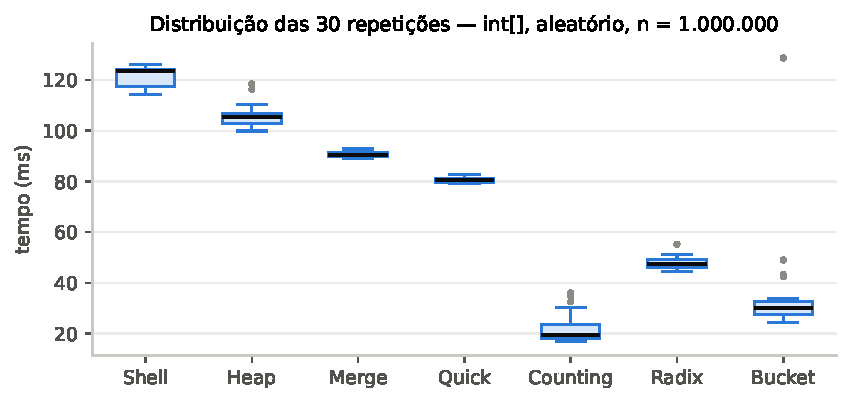
\includegraphics[width=0.88\linewidth]{fig_box_int_1M.pdf}\\[4pt]
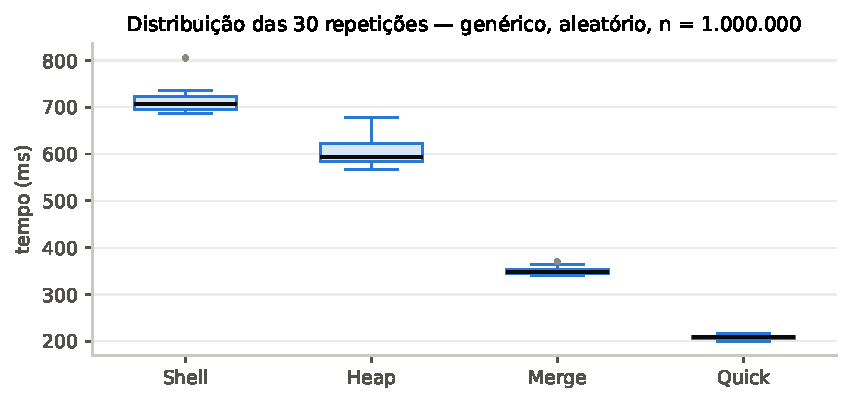
\includegraphics[width=0.88\linewidth]{fig_box_gen_1M.pdf}
\caption{Distribuição dos tempos das 30 repetições, ordem aleatória, $n=10^6$: \texttt{int[]}
(acima) e genérico (abaixo).}\label{fig:box}
\end{figure}

\subsection{Versão genérica versus \texttt{int}}

A Figura~\ref{fig:gen-int} mostra quantas vezes a versão genérica é mais lenta que a versão
\texttt{int} com a mesma lógica.

\begin{figure}[htbp]\centering
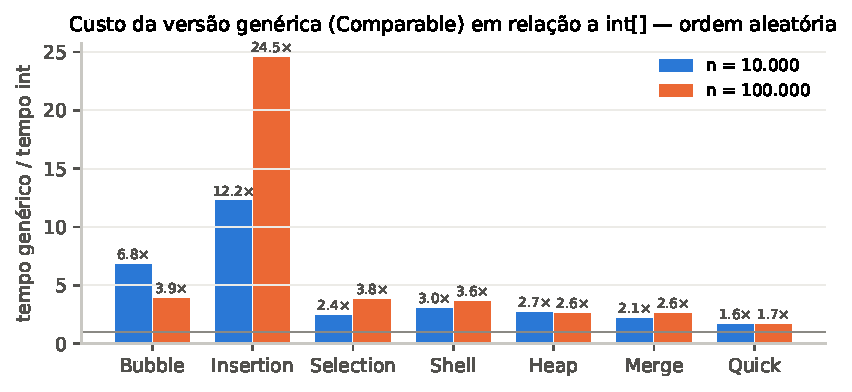
\includegraphics[width=0.88\linewidth]{fig_generico_vs_int.pdf}
\caption{Razão entre os tempos medianos das versões genérica e \texttt{int}, ordem aleatória.}\label{fig:gen-int}
\end{figure}

% ===============================================================
\section{Análise e discussão}
% ===============================================================

\subsection{Compatibilidade com as complexidades assintóticas}

\paragraph{Quadráticos.} O crescimento dos três métodos elementares é claramente quadrático: ao
multiplicar $n$ por 10 (de $10^4$ para $10^5$), o tempo do Insertion \texttt{int} passa de 5,81\,ms
para 596\,ms ($102\times$) e o do Selection \texttt{int} de 16,5\,ms para 1.780\,ms ($108\times$),
muito próximo do fator 100 previsto. Os expoentes empíricos são 2,01 e 2,02, e as curvas
normalizadas $t/n^2$ da Figura~\ref{fig:norm} são praticamente horizontais. O Bubble Sort
\texttt{int} se desvia (expoente 2,46): seu custo por operação quase triplica entre $n=10^4$ e
$n=10^5$. Uma explicação provável é a hierarquia de memória: o Bubble percorre o vetor inteiro a
cada passada e faz muitas escritas, e com $n \ge 5\cdot10^4$ o vetor (200--400\,KB) já não cabe nas
caches L1/L2 de um núcleo virtual que é compartilhado com o sistema hospedeiro. Não foi possível
confirmar essa hipótese com contadores de hardware dentro da máquina virtual. As versões genéricas
têm expoentes entre 2,19 e 2,32, também acima de 2 pelo mesmo motivo, agravado pelo fato de cada
\texttt{Integer} ser um objeto separado na memória.

\paragraph{$O(n\log n)$.} Quick e Merge Sort \texttt{int} têm expoentes 1,07 e 1,09, dentro da
faixa esperada para $n\log n$ (1,06--1,11), e suas curvas $t/(n\log_2 n)$ ficam estáveis em torno
de 4\,ns. O Heap Sort concorda com a teoria até $10^6$, mas em $n=10^7$ o custo normalizado
triplica. O motivo é o padrão de acesso: no heap, o filho de $i$ está em $2i+1$, então descer na
árvore significa saltar para posições cada vez mais distantes; quando o vetor (40\,MB) excede a
cache L3 (16\,MB), quase todo acesso nos níveis inferiores é uma falta de cache. O Shell Sort
apresentou expoente 1,16 (\texttt{int}) e 1,30 (genérico), coerente com o comportamento empírico de
aproximadamente $n^{1{,}25}$ da sequência de Knuth e abaixo do limite $O(n^{3/2})$.

\paragraph{Lineares.} Os lineares só se comportam como $\Theta(n)$ enquanto as estruturas cabem na
cache. Entre $10^4$ e $10^5$ o custo por elemento do Counting Sort fica constante (cerca de 5\,ns),
mas sobe para 22\,ns em $10^6$ e 92\,ns em $10^7$. Como $k=n$, o vetor de contagem cresce com a
entrada, e o incremento \texttt{c[a[i]]++} acessa posições aleatórias desse vetor: em $n=10^7$, são
40\,MB acessados aleatoriamente, e cada acesso custa o tempo de ir à memória principal. O Bucket
Sort sofre do mesmo efeito na distribuição dos elementos nos baldes. Já o Radix Sort tem custo por
elemento que cresce de forma gradual (de cerca de 35\,ns em $n=10^5$ para 59\,ns em $n=10^7$), e isso é previsto pela teoria nas nossas
condições: com valores até $n-1$, o número de dígitos $d = \lceil\log_{10} n\rceil$ cresce de 3 para 7.
Ainda assim, por fazer apenas passadas sequenciais, o Radix foi o mais rápido de todos em $n=10^7$
(593\,ms, contra 906\,ms do Quick Sort e 920\,ms do Counting Sort).

\subsection{Influência do tamanho do vetor}

O tamanho domina a diferença entre as famílias. Em $n=10^3$ todos os algoritmos levam menos de
1,5\,ms e a diferença entre o melhor e o pior é de cerca de 40 vezes (\texttt{int}). Em $n=10^5$
essa diferença passa de 18.000 vezes: o Bubble \texttt{int} leva 9,8\,s e o Counting Sort 0,5\,ms.
Para vetores pequenos os quadráticos são competitivos --- o Insertion \texttt{int} em $n=10^3$ (0,091\,ms)
fica na mesma ordem de grandeza dos $n\log n$ (0,046--0,076\,ms) --- o que justifica a prática de usar
Insertion Sort para subvetores pequenos em implementações híbridas.

\subsection{Influência da ordem da entrada (melhor, médio e pior caso)}

\paragraph{Insertion Sort.} É o caso mais didático. No vetor crescente o laço interno nunca executa
e o tempo cai para 0,012\,ms em $n=10^4$ ($\Theta(n)$), contra 5,81\,ms no aleatório. No decrescente
o número de deslocamentos é $n(n-1)/2$, o dobro do caso médio ($\approx n^2/4$), e o tempo medido é
1,96 vezes o aleatório em $n=10^4$ e 2,17 vezes em $n=5\cdot10^4$, em excelente acordo com a teoria.

\paragraph{Bubble Sort.} O melhor caso aparece como previsto: no vetor crescente a primeira passada
não faz trocas e o algoritmo para após $n-1$ comparações (0,012\,ms contra 35,4\,ms). O resultado
surpreendente é que, na versão \texttt{int}, o vetor decrescente --- teoricamente o pior caso, com o
número máximo de trocas --- foi \emph{mais rápido} que o aleatório (razão 0,62 em $n=10^4$ e 0,53 em
$n=5\cdot10^4$). A explicação está na \emph{previsão de desvios} do processador: no vetor
decrescente a comparação \texttt{a[j+1] < a[j]} dá quase sempre o mesmo resultado, e o processador
acerta a previsão; no aleatório o resultado é imprevisível, e cada erro de previsão descarta o
trabalho especulativo do pipeline. Na versão genérica, em que cada comparação é uma chamada a
\texttt{compareTo} com acesso a objetos na memória, esse efeito é menor que o custo das trocas, e
o decrescente volta a ser o mais lento (razão 1,14), como prevê a contagem de operações.

\paragraph{Selection Sort.} A teoria prevê o mesmo número de comparações em qualquer entrada, e
de fato crescente e aleatório têm tempos quase iguais (16,0 e 16,5\,ms). O decrescente, porém, foi
1,75 vez mais lento em $n=10^4$ e 5 vezes mais lento em $n=5\cdot10^4$. A diferença está na
atualização \texttt{min = j}: no vetor decrescente o mínimo muda em quase toda iteração da primeira
metade das passadas, criando uma cadeia de dependência (cada comparação precisa do valor de
\texttt{a[min]} recém-atualizado), enquanto no aleatório ele muda raramente. É um custo que a
contagem de comparações não captura; a interpretação é uma hipótese, pois depende do código de
máquina gerado pelo JIT, que não foi inspecionado.

\paragraph{Quick, Merge, Shell e Heap.} Com o pivô pela mediana de três, os vetores ordenados não
são o pior caso do Quick Sort: o pivô escolhido é exatamente a mediana e as partições ficam
perfeitamente equilibradas, o que torna o Quick de 2,5 a 4,5 vezes \emph{mais rápido} nos vetores
ordenados que no aleatório. Com o pivô fixo no primeiro elemento, a entrada ordenada levaria ao
custo $\Theta(n^2)$ e a uma recursão de profundidade $n$. O Shell Sort é o que mais ganha com
a entrada crescente (9,4\,ms contra 121\,ms em $n=10^6$), pois cada passada de inserção não
desloca nenhum elemento. O Merge Sort também acelera nos vetores ordenados (as intercalações
esgotam uma metade de cada vez, com desvios previsíveis), embora a teoria lhe atribua
$\Theta(n\log n)$ em todos os casos --- de novo, o número de operações é o mesmo, mas o custo de
cada operação muda. O Heap Sort é o menos sensível à ordem (razão 0,73).

\paragraph{Lineares.} Counting, Radix e Bucket praticamente não variam com a ordem em $n=10^4$
(razões entre 0,90 e 1,04), como prevê a teoria, já que o custo depende apenas de $n$ e dos
valores. Em $n=10^6$, porém, Counting e Bucket ficam duas vezes mais rápidos com entrada ordenada:
os acessos ao vetor de contagem e aos baldes passam a ser sequenciais, e a cache volta a ser
efetiva. O Radix Sort, que já acessa a memória de forma regular, não muda.

\subsection{Algoritmos com a mesma complexidade}

Há diferenças grandes entre algoritmos da mesma classe. Entre os quadráticos \texttt{int}, em
$n=10^5$, o Bubble (9,8\,s) é 16 vezes mais lento que o Insertion (0,6\,s), embora ambos sejam
$\Theta(n^2)$: o Insertion faz em média metade das comparações e desloca elementos com uma única
escrita por posição, enquanto o Bubble faz trocas completas (três atribuições). Curiosamente, na
versão genérica a ordem entre Insertion e Selection se inverte: o Selection, que faz no máximo
$n-1$ trocas, é o mais rápido, porque cada escrita de referência num \texttt{Integer[]} é cara
(ver Seção~\ref{sec:generico}).

Entre os $n\log n$, o Quick Sort foi o mais rápido em todos os tamanhos a partir de $10^4$. Em
$n=10^6$ a ordem foi Quick $<$ Merge $<$ Heap $<$ Shell nas duas versões; em $n=10^7$ o Heap Sort
passou a ser o mais lento. O Quick Sort tem o laço interno mais simples, opera no próprio vetor e
acessa a memória sequencialmente. O Merge Sort faz o mesmo número de comparações, mas copia cada
elemento para o vetor auxiliar a cada nível. O Heap Sort faz cerca de $2n\log n$ comparações e tem
acessos espalhados, e ficou três vezes mais lento que o Quick Sort em $n=10^7$.

\subsection{Custo da implementação genérica}\label{sec:generico}

A versão genérica foi de 1,6 a 24,5 vezes mais lenta que a versão \texttt{int}, com a mesma lógica
(Figura~\ref{fig:gen-int}). Três características da implementação explicam a diferença:
\begin{itemize}
  \item \textbf{Indireção}: um \texttt{Integer[]} guarda referências para objetos espalhados no heap;
        cada comparação precisa seguir duas referências e ler os valores, o que multiplica as faltas
        de cache. Um \texttt{int[]} guarda os valores contíguos.
  \item \textbf{Chamada a \texttt{compareTo}}: mesmo quando o JIT a otimiza, há mais instruções por
        comparação do que um simples \texttt{<} entre inteiros.
  \item \textbf{Barreira de escrita do coletor de lixo}: cada atribuição de referência a um vetor de
        objetos executa código adicional do coletor (marcação de \emph{card table}).
\end{itemize}
O caso extremo é o Insertion Sort ($24,5\times$ em $n=10^5$), que quase só faz deslocamentos
(\texttt{a[j+1] = a[j]}): na versão \texttt{int} esse laço é muito enxuto, e na genérica cada
deslocamento é uma escrita de referência com barreira. O Quick Sort é o menos penalizado
($1{,}7\times$), por fazer poucas trocas em relação às comparações. A lição é que a escolha
da representação dos dados pode pesar tanto quanto a escolha do algoritmo: o Insertion genérico
em $n=10^5$ (14,6\,s) foi mais lento que o Bubble \texttt{int} (9,8\,s).

\subsection{Variabilidade e confiabilidade}

Para as execuções longas a dispersão foi pequena: o CV ficou entre 1\% e 5\% para quase todos os
algoritmos em $n=10^6$ (Tabela~\ref{tab:det-int-1M}), e os boxplots mostram caixas estreitas. A
dispersão foi maior (i) em execuções muito curtas (menos de 1\,ms), mais sensíveis a interrupções
do sistema e à resolução do relógio; (ii) no Counting e no Bucket Sort em $n=10^6$ (CV de 25\% e
55\%), que alocam vetores auxiliares grandes a cada execução --- o tempo de alocação e de
mapeamento das páginas de memória varia, e uma única execução do Bucket Sort levou 129\,ms contra
mediana de 30\,ms; e (iii) no Quick Sort com vetor decrescente em $n=10^6$ (CV de 42\%), também por
causa de execuções isoladas lentas. Por isso a mediana foi usada nos gráficos. O fato de as
diferenças entre algoritmos serem muito maiores que a dispersão dentro de cada configuração dá
confiança às conclusões.

\subsection{Limitações}

\begin{itemize}
  \item As medições foram feitas numa máquina virtual com 2 vCPUs sobre um notebook com Windows;
        processos do sistema hospedeiro e a variação de frequência do processador podem ter afetado
        os tempos.
  \item Foi usado um único vetor aleatório por tamanho (semente fixa); repetições com sementes
        diferentes mediriam também a variação devida aos dados.
  \item Os quadráticos foram limitados a $n=10^5$ (ordem aleatória) e a $n=5\cdot10^4$ (ordenada e
        invertida), com 10 repetições nos maiores tamanhos, por restrição de tempo.
  \item Apenas uma distribuição de valores foi testada para os lineares ($[0,n)$ uniforme); com
        chaves de faixa maior ou distribuição concentrada, o Counting e o Bucket Sort teriam
        desempenho muito pior.
  \item As explicações baseadas em cache e previsão de desvios são compatíveis com os dados, mas
        não foram confirmadas com contadores de hardware.
\end{itemize}

% ===============================================================
\section{Conclusões}
% ===============================================================

Os experimentos confirmaram as ordens de crescimento previstas: expoentes empíricos de 2,0 a 2,5
para os métodos elementares e de 1,07 a 1,31 para os métodos $n\log n$, com o Quick e o Merge Sort
praticamente coincidindo com a curva $n\log n$. Os efeitos de melhor e pior caso também foram
observados com clareza, em especial no Insertion Sort ($\Theta(n)$ no vetor ordenado e o dobro do
caso médio no vetor invertido) e no Bubble Sort com parada antecipada. A escolha do pivô pela
mediana de três eliminou o pior caso do Quick Sort para entradas ordenadas.

Por outro lado, a complexidade assintótica sozinha não explicou os tempos observados. Algoritmos de
mesma classe diferiram por fatores de 3 a 16; o pior caso teórico do Bubble Sort foi mais rápido que
o caso médio na versão \texttt{int}, por efeito da previsão de desvios; e os algoritmos lineares
deixaram de ser lineares quando suas estruturas excederam a cache, com o Radix Sort --- que nessas
condições é na verdade $\Theta(n\log n)$ --- superando o Counting Sort em $n=10^7$. Os
algoritmos lineares foram os mais rápidos em quase todos os cenários, mas essa vantagem vale apenas
sob as condições adotadas (inteiros não negativos com $k=O(n)$ e distribuição uniforme).

Por fim, a extensão mostrou que a abstração genérica com \texttt{Comparable} tem custo
significativo em Java, de 1,6 a 24 vezes, por causa da indireção, das chamadas a
\texttt{compareTo} e das barreiras de escrita do coletor de lixo. Para dados primitivos em grande
volume, implementações especializadas compensam; para tipos arbitrários, a versão genérica oferece
flexibilidade, e o Quick Sort é o algoritmo menos penalizado por ela.

\section*{Dados e código}
Todo o código-fonte, os 3.850 tempos individuais (\texttt{resultados/tempos.csv}), as estatísticas
e o script de análise acompanham este relatório. O script \texttt{roda\_experimentos.sh} reproduz o
plano experimental completo.

\begin{thebibliography}{9}
\bibitem{cormen} T. H. Cormen, C. E. Leiserson, R. L. Rivest e C. Stein. \emph{Algoritmos: Teoria e
Prática}. 3.\,ed. Rio de Janeiro: Elsevier, 2012.
\bibitem{sedgewick} R. Sedgewick e K. Wayne. \emph{Algorithms}. 4.\,ed. Addison-Wesley, 2011.
\bibitem{knuth} D. E. Knuth. \emph{The Art of Computer Programming, Vol. 3: Sorting and Searching}.
2.\,ed. Addison-Wesley, 1998.
\end{thebibliography}

\end{document}
